%
%
%
\documentclass[twoside]{wiss}

\usepackage{graphicx}
\usepackage{nidanfloat} %% appended in WISS2010 for Future Vision (2010/7/7:akita)
\usepackage{multicol}
\usepackage{here} % [H]とするとその場所に配置されるらしい
\usepackage{color}

%% balance.styを追加 (2012/9/27:watanabe, Igarashi)
\usepackage{balance}    %% 最後のページの高さを揃えるために追加  (2012/9/27:watanabe, Igarashi)
%%% 最後のページの2段組の高さを揃える.\balanceを入れる.
%%% そろえたくないときは,\nobalance

\def\GEAR{\textsf{Gear}}
\def\GB{\textsf{GearBrowser}}
\def\figwidth{50mm}

\def\up{ 
\includegraphics[width=3mm,bb=0 0 36 36]{figures/uptriangle.pdf} }
\def\down{ 
\includegraphics[width=3mm,bb=0 0 36 36]{figures/downtriangle.pdf} }
\def\right{ 
\includegraphics[width=3mm,bb=0 0 36 36]{figures/righttriangle.pdf} }
\def\left{ 
\includegraphics[width=3mm,bb=0 0 36 36]{figures/lefttriangle.pdf} }
\long\def\comment#1{}

\journalhead{「超」ナビゲーション}

\begin{document}

\title{「超」ナビゲーション}
\etitle{} %2012年では英文タイトルは廃止されました.記入しないでください
% Supernavigation

% \author{増井 俊之\affil{Toshiyuki Masui, 慶應義塾大学 環境情報学部}}
\author{■■ ■■\affil{■■■ ■■■}}

\begin{abstract}
単純な装置で大規模な階層データを効率的にナビゲーションする手法を提案する。
%
% ファイルシステムや住所のような
大規模な階層データから項目を選ぶ場合、
% 階層を上下に移動したり同じ階層内の選択項目を移動したりするのが普通である。
階層を移動したり階層内の選択項目を移動したりすることによって目的の項目を検索するのが一般的である。
たとえば日本の住所リストから「□□県〇〇市△△」を検索する場合、
都道府県リストから□□県を選択し/□□県の市町村リストから〇〇市を選択し/
といった操作を繰り返して目的の項目に到達する。
別の県や市町村の住所を選択する場合は上位層に移動してから同様の操作を行なう。

このようなナビゲーションを行なうためには、
階層を上下に移動する手段と階層内を移動する手段が必要になるため、
3個以上のキーが用いられるのが普通である。
%
本論文では、2個のキーだけを使って
階層データのナビゲーションを実現する手法「{\GEAR}」を提案する。
{\GEAR}では
(1)階層内の項目選択時に端まで来た場合は上の階層に移動する.
(2)選択中の項目に下位階層がある場合は一定時間後に下の階層に移動する.
という手法により、
階層を上下に移動するためのキーが不要になり、
2個のキーだけであらゆる階層データを効率的にナビゲーションすることが可能になる。
\end{abstract}

\maketitle

\section{はじめに}

% 大量のデータを扱うために階層的に整理する手法がよく利用されている。

Web、
ファイルシステム、
住所のような
大規模データの多くは階層構造として表現されており、
階層構造を利用して情報を検索するインタラクション手法が広く利用されている。
階層的なデータを扱うための様々な情報視覚化手法が提案されているが
(\cite{Johnson:1991:TSA:949607.949654}\cite{Lamping:1995:FTB:223904.223956}\cite{Stasko:2000:FDN:857190.857683}\cite{Perlin:1993:PAA:166117.166125}など)、
これらはまだ一般的には普及しておらず、
現在のパソコンや携帯機器では、
シンプルなマウス操作やキー操作で階層構造をたどる手法が広く使われている。
%
例えばMacのファインダ\footnote{
  Macのデスクトップ画面でファイルを操作するための常駐基本ソフトウェア
}では、
ファイルの階層構造を視覚化/ナビゲーションするために
複数の手法が用意されており、
マウス/キー操作で階層型ファイルシステムのナビゲーションを行なうことができるようになっている。

パソコンや携帯機器のキーやボタンを利用して階層構造データのナビゲーションを行なう場合、
階層を上下に移動したり、
項目のリスト内を移動したりすることによって目的の情報を捜すのが普通である。
たとえばMacのファインダでは
上下矢印キーを使ってファイルやフォルダを選択したり、
左右矢印キーを使って階層を移動したりすることによって
目的のファイルに到達できるようになっている。

このような手法でナビゲーションを行なうためには、
通常3個以上のキーやスイッチが必要になる。
%
ファインダやテレビのリモコンなどでは
上下左右4方向のキーで階層データのナビゲーションを行なうようになっている。
またジョグダイヤルを登載した携帯電話や携帯端末では、
ダイヤルを回す操作とダイヤルを押す操作を組み合わせて
項目を選択したり階層を移動したりするものが多い。
%
一方、2個のスイッチだけで階層情報のナビゲーションを実行することができれば、
4方向キーや押しボタンつきジョグダイヤルなどよりも単純な装置を使って
階層情報のナビゲーションが可能になり、
いつでもどこでも誰でも簡単にデータを検索することができるようになる可能性がある。
%
本論文では、2個のスイッチだけを使って
階層構造を効率的にナビゲーションする「{\GEAR}」システムについて述べる。

\section{{\GEAR}のナビゲーション}
\label{description}

以下のような階層をもつファイルシステムのナビゲーションを考える。

\begin{figure}[H]
\centerline{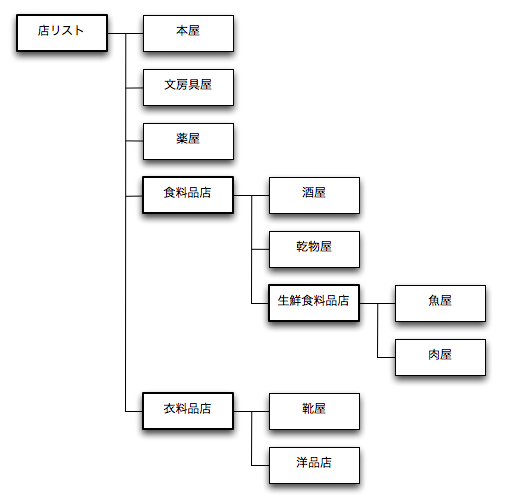
\includegraphics[width=70mm,bb=0 0 509 502]{figures/ae9216b00626f9c4eea44cc380f25886.png}}
\caption{階層的に表現されたショッピングモールの店リスト}
\label{screenshot1}
\end{figure}

\subsection{ファインダの階層情報ナビゲーション}

Macのファインダでは
{\up}{\down}{\left}{\right}という4個の矢印キーで
ファイルシステムのナビゲーションを行なうことができる。

「店リスト」をファインダで表示して「本屋」を選択すると、表示は以下のようになる。

\begin{figure}[H]
\centerline{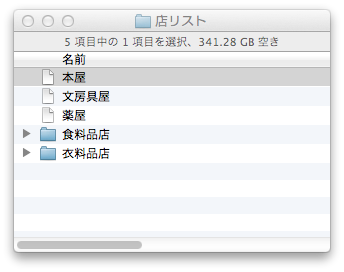
\includegraphics[width=\figwidth,bb=0 0 344 272]{figures/9b121bec45e5b480e5ac64fdd0f82592.png}}
\caption{店リストから「本屋」を選択}
\label{screenshot2}
\end{figure}

\noindent
ここで{\down}を押すと、次の「文房具屋」が選択される。

\begin{figure}[H]
\centerline{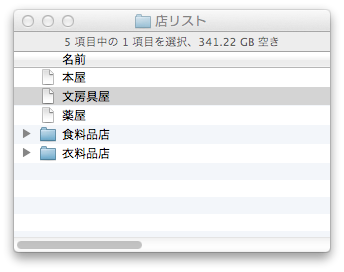
\includegraphics[width=\figwidth,bb=0 0 344 272]{figures/f43016d1b524baf414f2c32c48fe9588.png}}
\caption{ssss}
\label{「文房具屋」を選択}
\end{figure}

\noindent
さらに二回{\down}を押すと、以下のように「食料品店」が選択される。

\begin{figure}[H]
\centerline{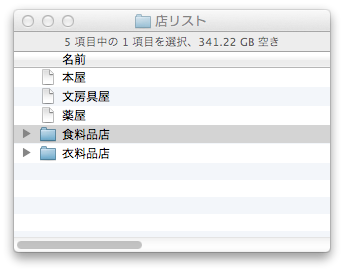
\includegraphics[width=\figwidth,bb=0 0 344 272]{figures/c074cd6daec3da0341125d1492b8a09c.png}}
\caption{「食料品店」を選択}
\label{screenshot4}
\end{figure}

\noindent
「食料品店」は下位階層を持っているので、
ここで{\right}キーを押すと
図\ref{screenshot5}のように下位階層が表示される。

\begin{figure}[H]
\centerline{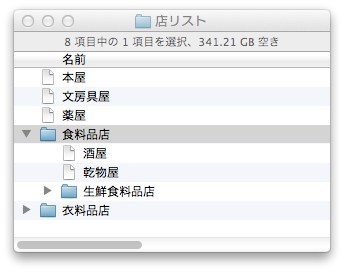
\includegraphics[width=\figwidth,bb=0 0 344 272]{figures/51d867d4721f65c18e84172c8818e137.png}}
\caption{「食料品店」の下位階層を展開して表示}
\label{screenshot5}
\end{figure}

\noindent
ここで{\down}キーを押すことによって「酒屋」を選択したり、
「生鮮食料品店」を選択してから{\right}を押すことによって、
さらに下位階層を表示することができる。

\begin{figure}[H]
\centerline{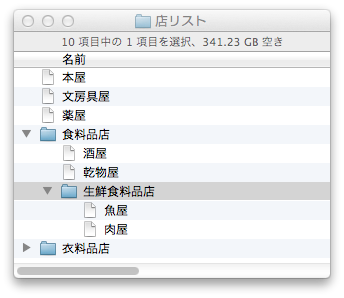
\includegraphics[width=\figwidth,bb=0 0 344 298]{figures/ce3ee682612de44d6c663a7323c262a6.png}}
\caption{「生鮮食料品店」の下位階層を表示}
\label{screenshot6}
\end{figure}

\noindent
また、この状態で{\left}キーを押すと下位層の表示を消し、
図\ref{screenshot5}の状態に戻すことができる。

このように、Macのファインダでは4個のキーを使って
階層データのナビゲーションを行なうことができる。
テレビのリモコンやジョグダイヤルでもほぼ同様の手法が利用されている。

\subsection{{\GEAR}によるナビゲーション}

{\GEAR}では{\up}と{\down}というふたつのキーだけを
利用してナビゲーションを行なう。

{\GEAR}で「店リスト」を表示すると、
ファインダの場合と同じように
図\ref{screenshot2}のようなリストが表示される。
{\down}を3回押すと
図\ref{screenshot42}のように「食料品店」が選択されるが、
そこで操作を中断して一定時間待つと「食料品店」の下位層が自動的に展開されて、
図\ref{screenshot7}のようにその最初の要素が選択される。

\begin{figure}[H]
\centerline{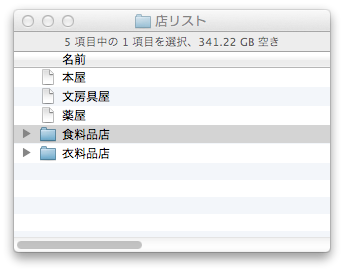
\includegraphics[width=\figwidth,bb=0 0 344 272]{figures/c074cd6daec3da0341125d1492b8a09c.png}}
\caption{「食料品店」を選択}
\label{screenshot42}
\end{figure}

\begin{figure}[H]
\centerline{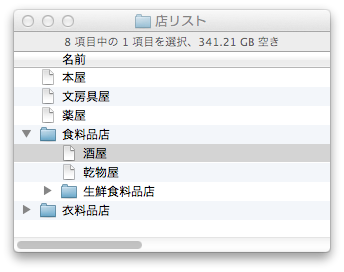
\includegraphics[width=\figwidth,bb=0 0 344 272]{figures/2387e402f81dbe7917e04df82b0a659c.png}}
\caption{「食料品店」の下位階層を自動展開}
\label{screenshot7}
\end{figure}

\noindent
ここで{\down}を2回押して「生鮮食料品店」を選択したまま一定時間待つと、
図\ref{screenshot8}のように
下位層が自動的に展開され、最初の要素である「魚屋」が選択される。

\begin{figure}[H]
\centerline{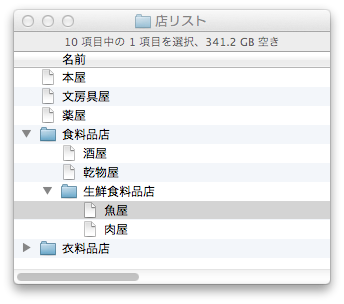
\includegraphics[width=\figwidth,bb=0 0 344 304]{figures/1b1955309d3baefda8e1b614cf06df62.png}}
\caption{「生鮮食料品店」の下位階層を自動展開}
\label{screenshot8}
\end{figure}

\noindent
つまり、{\right}のようなキーを押さなくても、
一定時間待つことによって同様の効果が得られることになる。

図\ref{screenshot42}のように食料品店を選択した状態から
時間を置かずに{\down}を押すと、
下位層は展開されず、次の「衣料品店」が選択される。

\begin{figure}[H]
\centerline{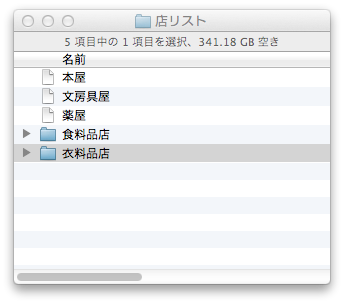
\includegraphics[width=\figwidth,bb=0 0 344 304]{figures/c5c757d8f79d5a8a9c85eef25600ba66.png}}
\caption{「衣料品店」を選択}
\label{screenshot9}
\end{figure}

\noindent
ここで操作を止めて一定時間待つと
下位層が自動的に展開されて「靴屋」が選択される。

\begin{figure}[H]
\centerline{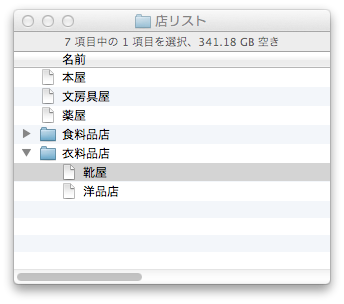
\includegraphics[width=\figwidth,bb=0 0 344 304]{figures/fddd5777d39924ea3f0220ae39a604c1.png}}
\caption{「靴屋」を選択}
\label{screenshot10}
\end{figure}

図\ref{screenshot8}の状態から{\up}キーを押すと、
下位層は自動的に閉じられて図\ref{screenshot7}の状態に戻る。 
さらに{\up}キーを押すと
「食料品店」の下位の層も閉じられ、図\ref{screenshot42}の状態に戻る。
%
また、図\ref{screenshot8}の状態から{\down}を2回押すと
「食料品店」の下位層は自動的に閉じられて図\ref{screenshot9}の状態になる。

まとめると、

\begin{enumerate}
\item \textbf{選択した項目に下位層が存在するときキー入力を行なわずに待つと下位層が自動的に展開され、下位層の最初の項目が選択される}
\item \textbf{項目リストの端を選択しているとき、さらに{\up}{\down}キーを押すと下位層は閉じられてひとつ上の層の項目が選択される}
\end{enumerate}

\noindent
というふたつの工夫により、
{\up}と{\down}だけで
階層データを自由にナビゲーションすることが可能になっている。

\section{実装}

ブラウザ上のJavaScriptで{\GEAR}を実装した
「{\GB}」を図\ref{gearbrowser}に示す。
ニュース・動画・音楽・電子書籍・、レシピ・地図など、
ブラウザで表示可能な多数のコンテンツの目次を{\GEAR}ウィンドウとして左側に表示し、
右側にコンテンツを表示している。

\begin{figure*}
\centerline{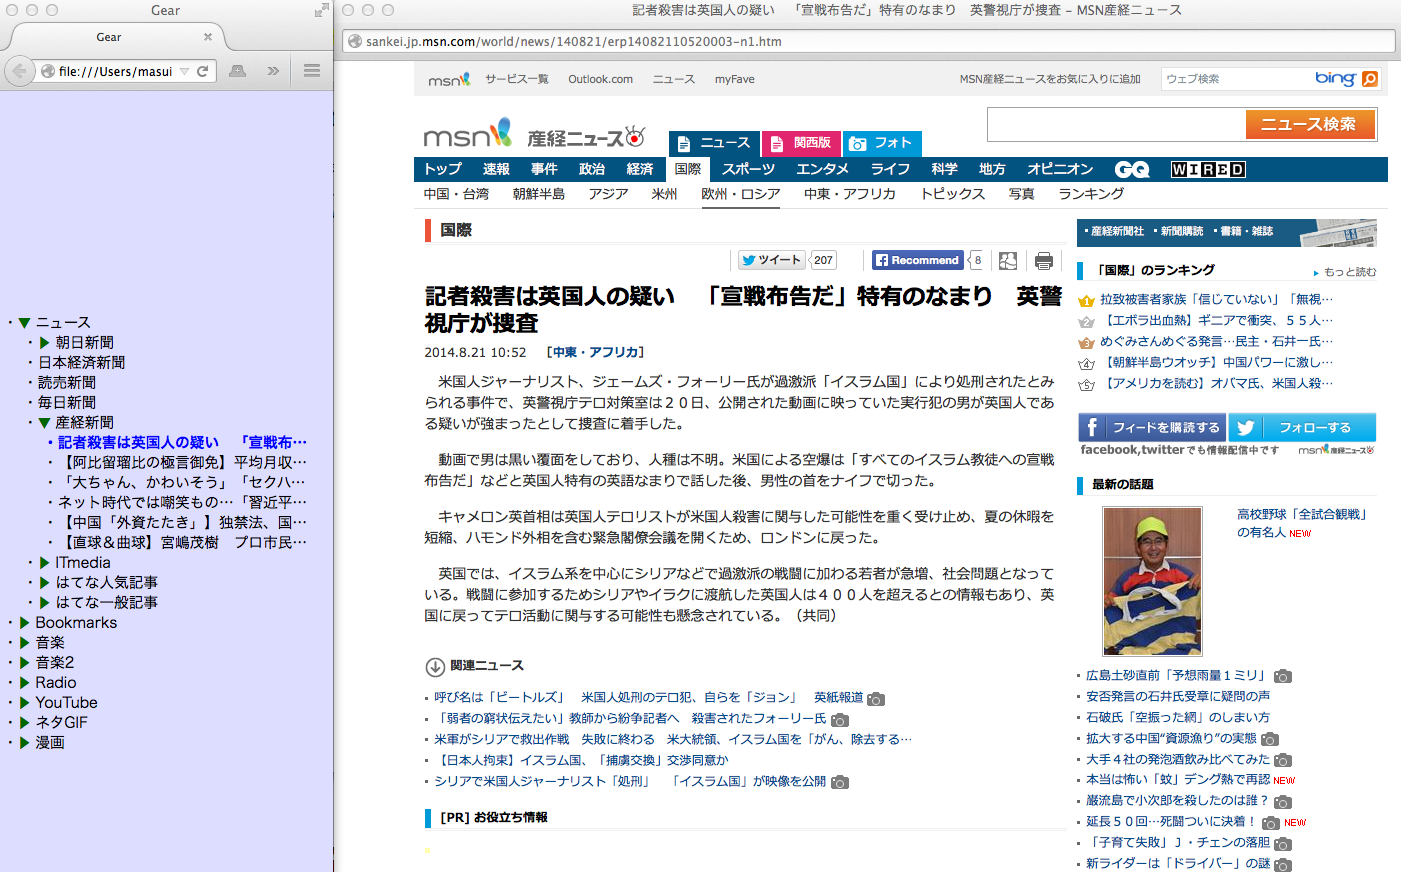
\includegraphics[width=160mm,bb=0 0 1401 872]{figures/ab4ff7c2d44f4af2bb94fae76589f495.png}}
\caption{\textsf{GearBrowser}}
\label{gearbrowser}
\end{figure*}

ユーザは{\up}と{\down}のみを使って{\GB}を操作する。
マウスホイールの回転も{\up}と{\down}に割り当てられているので、
ワイヤレスマウスをリモコンのように利用することができる。

著者のひとりは自宅の居間のテレビに接続したMac miniで{\GB}を半年以上利用している。
自宅にデジタル地上波が届かないこともあり、
{\GB}だけを利用して各種のコンテンツを楽しんでいる。

\section{議論}

\subsection{適用可能なデータのサイズ}

\ref{description}節では小さな階層データを利用して{\GEAR}の動作の説明を行なったが、
{\GEAR}は巨大なデータでも扱うことができる。
少なくともファインダで扱えるサイズのデータであれば
{\GEAR}でナビゲーションが可能である。
%
筆者宅の{\GB}ではすべての青空文庫コンテンツや1万本以上のアニメ動画を
{\GEAR}で選択して閲覧している。

%   普通にあらゆるデータに使えるといえるだろう
%   10レベルで6階層あれば10\^6のコンテンツに対応できるとか

\subsection{入力装置}

% 1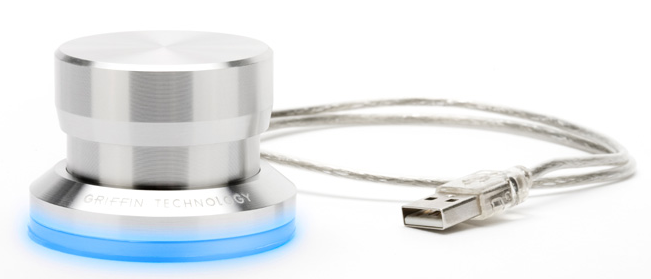
\includegraphics[width=50mm,bb=0 0 651 279]{figures/4a5e6e583649280eb4e0b3a0a8473b56.png}

{\GEAR}の操作は{\up}{\down}というふたつの入力しか必要としないため、
圧力センサや回転ダイヤルなどを利用した各種の実装が可能である。
%
図\ref{disk}は、回転円板による{\GEAR}の実装である。
左右の回転を{\up}{\down}に割り当てている。

\begin{figure}[H]
\centerline{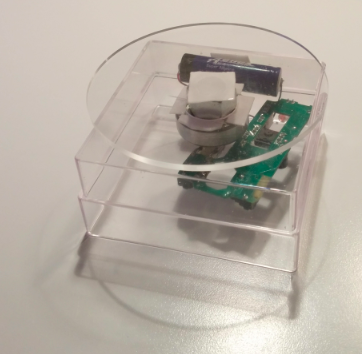
\includegraphics[width=50mm,bb=0 0 362 354]{figures/ff2d18e66f9a4655dbb5e22e0bb9a0ae.png}}
\caption{回転板}
\label{disk}
\end{figure}

図\ref{paddle}は、
パドルに貼った2個の圧力センサの値を{\up}{\down}に割り当てている。

\begin{figure}[H]
\centerline{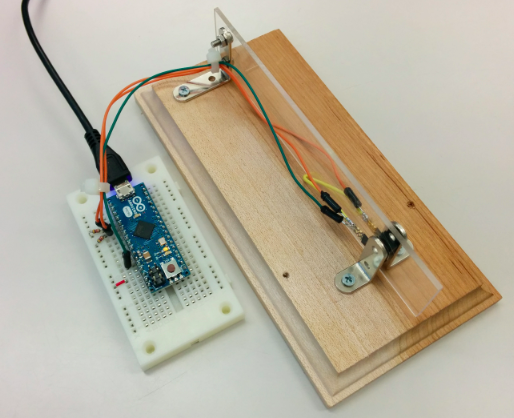
\includegraphics[width=50mm,bb=0 0 514 418]{figures/3c2de63899653056f3c6be835b9aaf43.png}}
\caption{左右にはじく「パドル」デバイス}
\label{paddle}
\end{figure}

\noindent
このように、現状のGUIでは利用されていないようなデバイスでも
{\GEAR}の入力装置として利用することができる。

\subsection{操作の量}

図\ref{screenshot2}の状態から
図\ref{screenshot8}の状態に移動する場合、
Macのファインダでは9回キー操作を行なう必要があるが
{\GEAR}では5回だけでよい。
{\GEAR}では下位層に移動するのに時間待ちが必要なので操作全体にかかる時間は大差ないが、
操作の数は少なくてすむので、
運動障害のあるユーザや機器の操作が難しい環境において有効と考えられる。

\subsection{扱えるデータ構造}

辞書のようなフラットなデータは読みや綴りで階層的に分類できるし、
時刻情報のような連続的なデータでも
年/月/日のように階層化して管理することができる。
また、SNSの友達関係のようなネットワーク構造をもつデータも
木構造的に表現することが可能なので、
ほぼあらゆるデータは木構造で表現可能であり、
{\GEAR}で扱うことが可能である。

% \subsection{想定される利用者}
% 
% 著者のひとりは{\GEAR}を通常の家庭環境で利用しているが、
% 
%   はっきり言って、ほとんど誰でも使えると思う
% 
%   Unixでよく使うコマンドは cd, ls, more とかである
%   FinderとかExplorerとかの基本ソフトで使う
%   これ以外にはキーワード検索とかもあるけど

\subsection{階層構造の構成}

同じ階層に沢山の項目が含まれている場合、
{\up}や{\down}によるナビゲーションが難しい場合がある。
たとえば、電子書籍のすべての著者を同じ階層に並べてしまうと
著者リストの中から{\up}{\down}で著者を選択するのは困難である。
著者名の読みを「あ」から「わ」までで分類することによってひとつ階層を増やすと事態は改善されるが、
{\up}{\down}で五十音を選択するのにはやはり時間がかかる。
この場合は、「あ行」「か行」のような大分類の下に「あ」「い」「う」のような小分類の階層を作成し、
その下に著者名を並べる方が効率が良いだろう。

このように{\GEAR}でナビゲーションする階層データは構成に注意する必要があるが、
通常のファイルシステムやURLの階層構造でも同様の問題は存在する。
{\GEAR}の場合、装置の制約が大きいため階層構造についてより細かな注意が必要だといえるだろう。

\subsection{ザッピング}

% 決定ボタンを押す方式だと、単に回転するだけでは次のページに移ることができない
%   下矢印だけで次頁に移動できる!
%   最下位の層でザッピングできる
%   単に「次」を押していけば漫画や順番に
%   「前」の場合はそうはならないが、「次」の方が圧倒的に多いはずだから大丈夫

{\GB}では、コンテンツを単純な操作で連続的に楽しむことができる。

\begin{figure}[H]
\centerline{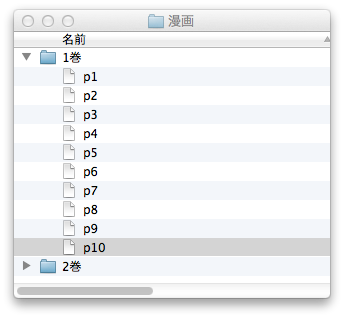
\includegraphics[width=\figwidth,bb=0 0 344 318]{figures/9a8615b0242c9ba4deb77ca30ab94d7c.png}}
\caption{1巻の最終ページ}
\label{manga1}
\end{figure}

\noindent
図\ref{manga1}のような漫画の1巻の最終ページから
次の巻の最初のページに移りたいとき、
ファインダのように上下左右キーを利用する場合は

\begin{itemize}
\item {\left}で1巻を閉じる
\item {\down}で2巻を選択する
\item {\right}で2巻の要素を開く
\item {\down}で2巻の先頭要素を選択する
\end{itemize}

\noindent
という操作が必要であるが、{\GB}では

\begin{itemize}
\item {\down}を押す
\end{itemize}

\noindent
だけでよい。
図\ref{manga1}の状態で{\down}を押すと
1巻の下位要素は閉じられ、
2巻の下位要素が自動的に開いて最初の要素が表示されるからである。

つまり、{\GB}では
何も考えずに
{\down}を押すだけでコンテンツを順番に楽しむことができることになる。
何も考えずに単純な操作を繰り返すだけでコンテンツを検索できるということは
従来のテレビのチャンネルを回す「ザッピング」と似ており、
能動的に計算機を利用することが不得手なユーザでも
利用しやすいと考えられる。

% そもそも姿勢が違うのである
% 前かがみになって入力装置を操作するのはテレビには向いいない

\subsection{音声の利用}

{\GEAR}は階層構造を表示しながら利用するのが基本であるが、
項目を選択したときタイトルを読みあげることにより、
階層構造を表示せずにナビゲーションを行なうことが可能である。
この場合は階層の構造についてあらかじめ知っておくことが望ましいが、
表示装置を利用できない状況でも
音楽コンテンツなどを選択可能になるので便利である。

% \subsection{操作が超シンプルだというのはどういうことか}
% 
% かなりの運動障害があっても使える
% 操作が少ないので、誰でも試行錯誤でなんとかなるだろう
% 一方、筆者は毎日食卓から{\GEAR}を使ってニュースを見たり音楽を聞いたりしている
% 障害があってもなくても同じように便利だというのが理想である

% \subsection{ひとつの階層に沢山のデータを置いてはいけない。スクロールの速度にもよるが、20個以下程度が妥当と思われる。}
%    読みの場合は「あ」「か」「さ」

% \subsection{どういうデータに使えるか}
% 
%    {\GEAR}は木構造にしか適用できない
%    専門的に管理されているデータは木構造が多く、
%    そうでないものはタグなどを利用してネットワーク構造にするのが良いと思われる
%    あらゆるネットワーク構造は木構造に変換可能だし
%      表型式でも木構造の一種と考えることができる
%      Cでは「配列の配列」が「表」だが
%    同じデータがあちこちに出てきてもよい
%      日付による分類とキーワードによる分類

% \subsection{障害対応}
% 
% 「障害者」用の装置を作っては駄目で、障害が有ってもなくても使える装置を作るべきだろう。

% 同様に、初心者用/老人用/子供用のシステムを作るよりも、初心者でも老人で
% も子供でも使えるシステムを作る方がスジが良いと思う。

\subsection{時間待ちについて}

{\GEAR}では、下位層が存在する項目を選択した状態で時間待ちすると
その項目を選択して下位層を展開するようになっているが、
時間によって動作が変わることを気にするユーザは多いようである。
%
一般に、タイミングによって挙動が変わるインタフェースは望ましくないと考えられているが、
操作の量を減らすためにタイミングを利用することに意味がある場合がある。
例えば、運動に関する重度な障害がある人の場合、
操作のタイミングを利用して文字入力を行なう「スキャン入力」のような
手法は広く利用されている\footnote{
  \textsf{http://www.resja.or.jp/com-gl/gl/a-1-1.html}
}。
% このような手法は「障害者」用のものだと考えられているかもしれないが、
入出力装置に制限がある場合のトレードオフとして
時間情報を利用することは意味があると考えている。

% ALS用文字入力システムではタイミングで選択操作を行なっている
%   何と呼ぶのだっけ?
%   腕は自由に動かないが、あるタイミングで腕を動かすことは可能だというタイプの障害が存在し、
%     そういう症状は多い
% e.g. Pete

% \subsection{選択以外の操作}
% 
% 普通のWebページだとスクロール操作が必要になるが
%   スクロールはなんとか大丈夫
%   早送りとかは工夫が必要
%     だけどできる
% 音量や画面の明るさ調整などは別操作が必要になるだろう
%      これは別のチャンネルを利用すべきかもしれない
%      別になっている方が一般に望ましいだろう
%        だからiPhoneでもAndroidでも音量だけは別操作になっていてメニューで選んだりしない

\subsection{{\GEAR}が有効な状況}

{\GEAR}によるナビゲーションは
パソコン上でマウスやキーボードを利用するナビゲーションよりも遅いことは間違いないが、
マウスやキーボードに比べると装置が圧倒的に単純で良いため、
そういった装置を使いにくい環境で利用することに意味があるだろう。
ユビキタスコンピューティング時代には、
パソコンで一般的な入力装置を使えない場合の方が多いと思われるため、
{\GEAR}のような手法が有効である機会は多くなるだろう。

% \subsection{Lindaで実装}

\subsection{関連研究}

階層データのナビゲーション手法は長年広く利用されているが、
現在普及している手法よりも良い方法が有ると期待されていないためか、
本論文のような研究は長らく行なわれていないようである。
%
{\GEAR}はあまりにも単純な手法であるため、
同じ手法がこれまでに存在した可能性を否定することはできないが、
多くのHI研究者や開発者に感想や意見を求めた限りでは
{\GEAR}と同じ手法の存在は確認できていないので、
少なくとも近年に同様のシステムが存在した可能性は低いと思われる。
%
今のところ{\GEAR}が再発明なのか新発明なのか断言することはできないが、
このようなナビゲーション手法は
現在のユビキタスコンピューティング環境で最も必要とされる技術の
ひとつには違いないと思われる。

\section{結論}

非常に単純な入力装置を利用して大規模な階層構造データをナビゲーションする
手法「{\GEAR}」を提案した。
{\GEAR}の使い方は単純であり、
一度慣れてしまえば問題なく利用できる。

{\GEAR}のように実装も操作法も簡単で有用なシステムは、
誰もがいつでもどこでも計算機やネットワークを活用する
ユビキタスコンピューティング社会において
重要な存在になるであろう。

{\scriptsize
\bibliographystyle{jwiss}
\bibliography{paper}
}

\end{document}


